\chapter{Conception}

Les données brutes sur lesquelles le pipeline d'analyse est développé ont déjà subi une étape de pré-traitement durant laquelle les adaptateurs et les séquences d'une qualité inférieure à 20 ont été supprimés et les séquences chevauchantes ont été scindées en deux parties. Ces données ainsi nettoyées ont été alignées et servent d’entrées pour le pipeline d'analyse. Le développement du pipeline d'analyse se focalise donc sur la détection de variants. 

Lors de ce stage, les variations des TFBS doivent être isolées du reste des données. L'extraction de ces variations implique le développement d'un pipeline d'analyse. Il commence par une réorganisation des données afin de limiter les erreurs liées au séquençage et à l'alignement des séquences.

Les pipelines d'analyses spécifiques aux données NGS se construisent suivant un ordre précis décrit dans la publication de \citet{ref7}.

Quatre grandes étapes sont indispensables lors de l'analyse des données :
\begin{itemize}[label=\textbullet]
\item Organiser les données
\item Détecter les variants
\item Annoter les variants
\item Filtrer les résultats 
\end{itemize}

La figure \ref{fig:pipeline} ci-dessous, illustre le pipeline d'analyse élaboré, dans le but d'extraire toutes les variations des TFBS des différents échantillons de LMS disponibles. 

\begin{figure}[h]
\centering
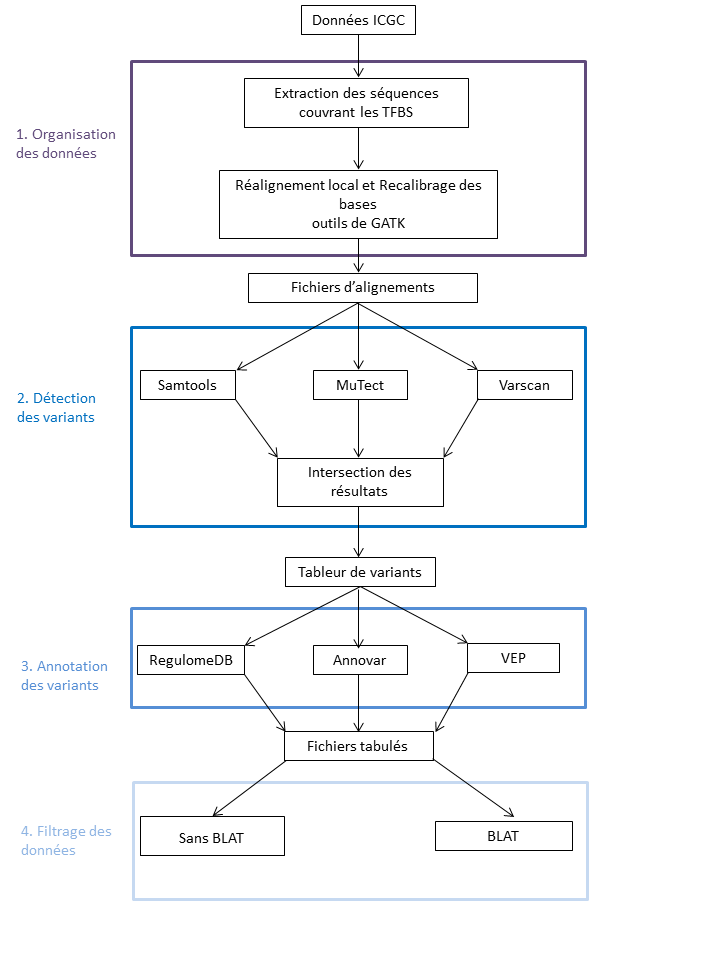
\includegraphics[width=10cm,height=11cm]{Figures/pipeline.png}
\caption{Pipeline d'analyse des données de l'ICGC}
\label{fig:pipeline}
\end{figure}

\section{Organisation des données}\label{sec: orga}

Les données issues de techniques de séquençage NGS de génomes complets sont très volumineuses, il est donc intéressant de les scinder en fonction des besoins. La figure \ref{fig:part1} montre la première partie du pipeline d'analyse. Dans cette partie les données seront extraites puis nettoyées.

\begin{figure}[h]
\centering
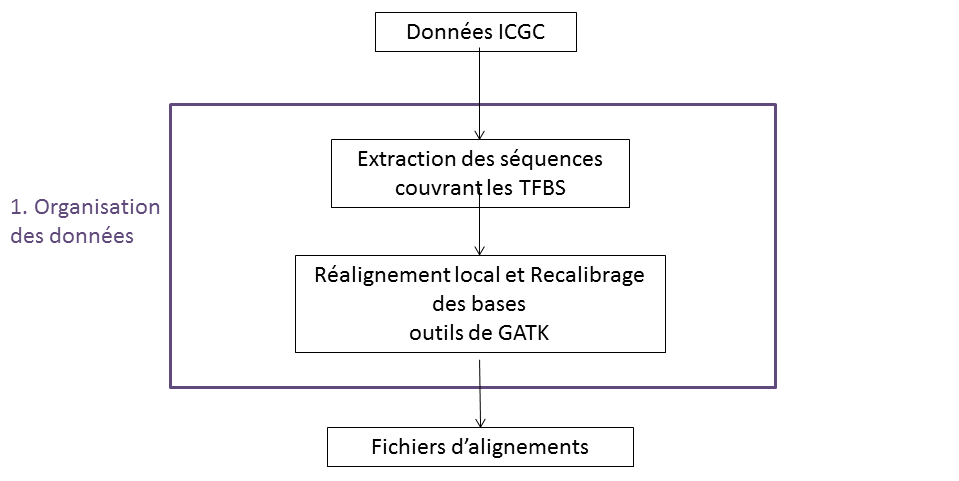
\includegraphics[scale=0.6]{Figures/partie1.png}
\caption{Réorganisation des données}
\label{fig:part1}
\end{figure}

Dans le cadre de ce projet de stage, je focaliserai mes analyses uniquement sur l'étude des TFBS. L'outil \textit{\textbf{view}} du logiciel \textbf{Samtools} pourra être utilisé pour extraire les séquences qui les recouvrent du reste du fichier d'alignement. Les options -H et -R sont passées en paramètres.

Les \og read group\fg ~n'ont pas été ajoutés lors de l'alignement des séquences (pas d'utilité pour l'équipe au moment de leur génération) or ils sont nécessaires au fonctionnement de logiciels d'alignement (MuTect, Varscan). L'outil \textit{\textbf{AddOrReplaceReadGroups}} de \textbf{Picartools} semble être utilisable pour les ajouter. Dans le but d'accélérer le processus, les paramètres suivant pourraient être donnés en entrées VALIDATION\_STRINGENCY = SILENT pour éviter les tests de validation des séquences, SORT\_ORDER = coordinate pour trier le fichier de sortie suivant ses coordonnées et CREATE\_INDEX = True pour créer un index du fichier de sortie.

Un second outil du même logiciel, \textit{\textbf{ReorderSam}}, pourra être mis à contribution pour réordonner les fichiers dans l'ordre caryotypique. Ce nouveau fichier ne sera pas indexé car l'utilisation de l'option qui le permet augmente le temps d'exécution. Pour l'indexer, l'outil \textit{\textbf{index}} du logiciel \textbf{Samtools} sera privilégié en raison de sa rapidité d'exécution.

Les fichiers réorganisés doivent passer par une étape de traitement supplémentaire pour éliminer le maximum d'erreurs liées au séquençage ou à l'alignement. Parmi tous les logiciels de manipulation des données présentés dans la partie \ref{subsec:manip}, un seul a été retenu : \textbf{GATK}. Les outils \textit{\textbf{RealigneTargetCreator}}, \textit{\textbf{IndelRealigner}}, \textit{\textbf{BaseRecalibrator}} et \textit{\textbf{PrintReads}} de ce logiciel pourront être mis à contribution lors de cette étape.

\newpage
\subsection{Le traitement par GATK}\label{sec: GATK}

Lors du séquençage, des erreurs liées à la technique utilisée ont pu être imprimées dans les fichiers de sortie. Il est donc important d'éliminer au maximum ces erreurs potentielles. Les concepteurs de GATK conseillent de passer les bases de données \textbf{Mills} et \textbf{1000G} aux outils \textit{\textbf{RealigneTargetCreator}} et \textit{\textbf{IndelRealigner}}. La base de données Mills est beaucoup plus restrictives que 1000G, elle ne sera donc pas conservées. La base de données 1000G peut être considérées comme robuste en raison du nombre important de données qui ont servis à la constituer bien que chaque donnée ne soit pas expérimentalement vérifiée. Elle sera donc conservée pour ces étapes.

Les erreurs liées au séquençage ne sont pas les seules, des erreurs liées à l'alignement des séquences peuvent exister. Les outils \textit{\textbf{BaseRecalibrator}} et \textit{\textbf{PrintReads}} de \textbf{GATK} pourront être mis à contribution pour les supprimer. Il est conseillé de passer, en supplément des deux bases Mills et 1000G, la base de données dbSNP dans une version supérieure à la 132. Pour les raisons citées dans le paragraphe précédent Mills n'est pas conservée. La base de donnée dbSNP contient un nombre très important de données cependant, toutes ces données n'ont pas été vérifiées expérimentalement. Du fait de cette information, cette base ne sera pas conservée. Ces outils disposent d'options de parallélisation (nombre de cpu, nombre de cœurs), elles pourront être prises en compte afin d'accélérer les processus d'exécution.

Des fichiers BAM ne contenant théoriquement plus d'erreur sont générés à la suite de ces deux étapes. Ces fichiers passent à l'étape suivante du pipeline : la détection des variants somatiques.

\section{Détection des variants somatiques}\label{sec:detec}

La seconde partie du pipeline est présentée dans la figure \ref{fig:part2}. Cette partie permettra de détecter les variants des TFBS.

\begin{figure}[h]
\centering
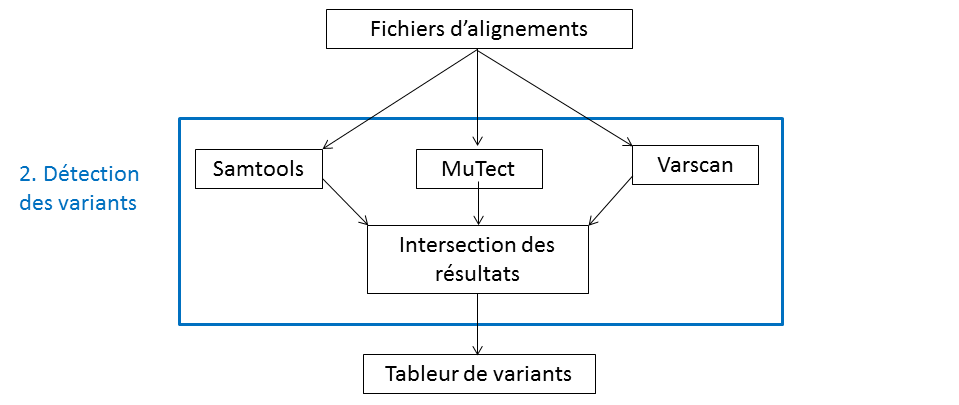
\includegraphics[scale=0.6]{Figures/partie2.png}
\caption{Détection des variants}
\label{fig:part2}
\end{figure}

Dans la partie \ref{subsec:caller} de l'analyse de ce sujet, plusieurs outils de détection de variants ont été examinés. Ces outils ne permettent pas tous de travailler simultanément sur plusieurs fichiers comme pour l'analyse comparative de données tumorales et constitutionnelles. 

\textbf{Atlas2} ne prend qu'un seul fichier en entrée, il ne peut donc pas comparer les séquences de l'échantillon tumorale avec celle de l'échantillon constitutionnel. Son utilisation nécessitant une étape de post-traitement, il ne sera pas conservé.

L'ensemble des données ayant déjà été généré avec \textbf{Samtools} par l'équipe, il sera conservé bien qu'il présente les mêmes caractéristiques qu'\textbf{Atlas2}.

\textbf{SomaticSniper} ne détecte que les SNP or pour analyser les variations des TFBS il faut également détecter les INDEL, il ne pourra donc pas être utilisé.

Une étude comparative de plusieurs outils de détection parmi lesquels se trouvent \textbf{Varscan} et \textbf{MuTect} \citep {Detecting} démontre que \textbf{Varscan} est le plus performant quand il s'agit de détecter des SNP de haute qualité (couverture et fréquence allélique prise en compte) et que \textbf{MuTect} au contraire détecte plus de SNP de basse qualité que les autres. Ces deux outils seront donc utilisés pour détecter les variants des TFBS. 

Les caractéristiques présentées dans le tableau \ref{caract} de l'analyse du sujet et les deux études précédemment citées permettent de sélectionner \textbf{MuTect} et \textbf{Varscan} comme logiciel de détection de variants pour la suite du pipeline. \textbf{Samtools} étant historiquement utilisé au sein de l'équipe et un certain nombre de données ayant déjà été calculées dessus, il m'a été demandé de l'intégrer comme un outil de mon pipeline.

\subsection{MuTect}

Lors de l'analyse du sujet, \textbf{MuTect} a été présenté comme comportant plusieurs filtres par défaut. Toutes les variations détectées ayant réussi à passer ces filtres sont étiquetées avec la valeur \og PASS\fg ~dans le champ \og FILTER\fg ~du fichier de sortie. Ces variations sont considérées comme somatiques. 

Le fichier de sortie est au format VCF, pour garder ce format il faudrait récupérer le header. L'outil \textit{\textbf{view}} du logiciel \textbf{Samtools} semble être applicable avec l'option -h pour extraire uniquement le header et le placer dans un fichier vide.

Dans le but de ne conserver que les variations somatiques, la commande \og grep \fg ~du shell linux pourrait être employée pour récupérer toutes les lignes étiquetées \og PASS\fg. Ces lignes seront conservées à la suite du fichier contenant le header, un nouveau VCF sera ainsi formé.

\subsection{Varscan}

Dans l'analyse du sujet, il est décrit que \textbf{Varscan} prend en entrée un seul fichier au format mpileup. Cependant, ce logiciel ne fournit aucun outil de transformation des fichiers BAM en mpileup. L'outil \textit{\textbf{mpileup}} de \textbf{Samtools} pourra être mis à contribution pour générer le fichier attendu. Les options -B pour supprimer le calcul de probabilité qu'une séquence soit mal alignée et -f pour donner la séquence de référence pourront être passées en entrées. L'option -q avec la valeur 1 qui permet de ne conserver que les séquence de qualité minimum 1 pourra également être utilisée.

Dans la partie \ref{subsec:varscan} il a été vu que deux fichiers VCF sont générés par \textbf{Varscan}. L'outil \textit{\textbf{ProcessSomatic}} pourra être mis en application sur chacun de ces fichiers afin de séparer les variations somatiques des autres variations LOH et germinales.

L'extraction va de nouveau produire quatre fichiers, deux pour les SNP, un avec les variations de haute qualité et un second avec les autres, et deux pour les INDEL, un avec les variations de haute qualité et un avec les autres. L'outil \textit{\textbf{vcf-concat}} du logiciel \textbf{VCFtools} pourra être utilisé afin de les rassembler en un seul fichier qui contiendra les SNP et les INDEL de haute qualité. Ce fichier pourra alors être fusionné avec celui généré par \textbf{MuTect}

\subsection{Samtools}\label{subsec:sam}

Le logiciel Samtools permet de faire de la détection de variants cependant il doit être associé à un autre logiciel, \textbf{BCFtools}.

Un pipeline de détection de variants réalisé avec Samtools a déjà été développé par l'équipe de l'institut Bergonié. Ce pipeline permet de détecter toutes les variations présentes dans un jeu de données. Cependant les variations détectées ne sont pas toutes somatiques. Il faudra donc appliquer des filtres sur les données obtenues. 

Les filtres qui seront utilisés ont déjà été développés par \cite{Filtre}. Dans cet article, les auteurs partent du principe qu'une variation est somatique si la couverture minimale de l'échantillon constitutionnel est de 8 et celle de l'échantillon tumoral de 14 à cette position. Les variations dont la fréquence allélique est supérieure ou égale à 30\% sont conservées. 

\section{Annotation des variants}

Le processus d'annotation des variants permet de caractériser les différentes variations détectées d'après le processus de la partie \ref{sec:detec}. Plusieurs outils ont été présentés lors de l'analyse de ce sujet. La troisième partie du pipeline présentée sur la figure \ref{fig:part3} montre le cheminement du processus d'annotation.

\begin{figure}[h]
\centering
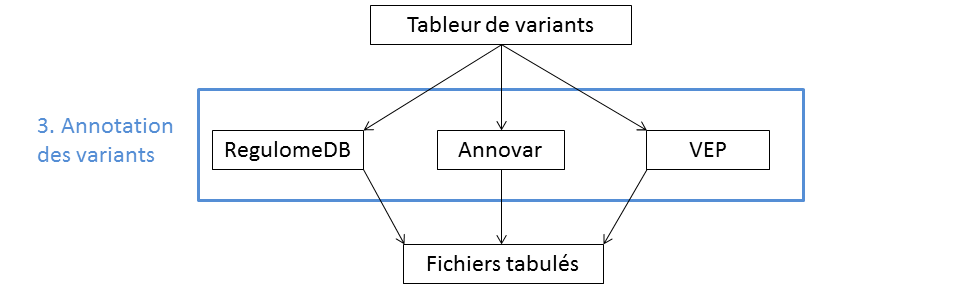
\includegraphics[scale=0.6]{Figures/partie3.png}
\caption{Annotation des variants}
\label{fig:part3}
\end{figure}

\subsection{Choix des logiciels}

Le logiciel \textbf{Annovar} permet d'utiliser de nombreuses bases de données lorsqu'elles sont formatées selon les exigences du logiciel. Il peut donc théoriquement utiliser n'importe quelle base de données. \textbf{Annovar} est très rapide, performant et régulièrement mis à jour. Il est donc retenu pour faire l'annotation des variants somatiques. Les scripts permettant de faire de l'annotation simple et multiple pourront être utilisés en fonction du nombre de base de données sélectionnées.

Le logiciel \textbf{VEP} est rapide et performant, il utilise des bases de données de transcrits comme \textbf{Gencode} pour annoter les variants. VEP peut détecter des variations dans les régions régulatrices, cependant il n'est pas possible de lui donner une base de données des TFBS, il ne détectera donc que ce qui se trouve dans les bases de données de transcrits qu'il utilise. Ce logiciel ne sera donc pas retenu pour réaliser l'annotation des variants somatiques des TFBS, il pourra cependant être utilisé pour annoter les transcrits.

Le logiciel \textbf{R} et son package \textit{\textbf{VariantAnnotation}} ne permettent d'utiliser qu'un nombre limité de base de données (SIFT et Polyphen), ils ne seront donc pas conservés pour annoter les variants.

L'outil \textit{\textbf{VariantAnnotator}} proposé par \textbf{GATK} annote les variants selon leur contexte. Il permet par exemple de ressortir la profondeur de couverture de chacun ou encore la fréquence allélique. Il ne permet en revanche pas d'annoter les variants avec une base de données, il ne sera donc pas conservé pour l'étape d'annotation des variants.

Le logiciel \textbf{Oncotator} développé par le \textit{Broad Institute} n'annote que les points de variations et les INDEL de petites tailles. Il présente l'avantage d'annoter les variants en fonction de leur nom et de produire des liens vers des données spécifiques du cancer. Cependant, cela implique que les variants détectés soient déjà connus or je ne peux en être sûre, c'est pourquoi je ne conserve pas ce logiciel.

\begin{table}[h]
\centering
\begin{tabular}{|c|c|c|c|c|}
\hline
Logiciel & Choix des bdd & TFBS & Fonctionnelle \\
\hline
Annovar & \textbf{OUI} & \textbf{OUI} & \textbf{OUI}\\
\hline
VEP & non & non & \textbf{OUI}\\
\hline
Oncotator & non & \textbf{OUI} & \textbf{OUI}\\
\hline
VariantAnnotator & \textbf{OUI} & \textbf{OUI} & non\\
\hline
VariantAnnotation & non & \textbf{OUI} & \textbf{OUI}\\
\hline
\end{tabular}
\caption{Récapitulatif du choix des logiciels d'annotation}
\end{table}

\subsection{Choix des bases de données}

L'application web \textbf{RegulomeDB} utilise une base de données \textbf{dbSNP} pour réaliser l'annotation des variants des régions régulatrices. Le format de RegulomeDB risque de rendre son utilisation très difficile si le nombre de variations est élevé, un script pourrait être réalisé afin d'utiliser l'application localement. Annotant toutes les régions régulatrices, cette base contient les TFBS et sera conservée.

La base de donnée des TFBS, \textbf{tfbsConsSites}, de l'\textit{UCSC} est formatée pour pouvoir être utilisée avec Annovar afin d'annoter les variations somatiques des TFBS. Toutes les données qui y sont intégrées doivent avoir été vérifiées expérimentalement auparavant, cette base est donc fiable bien qu'elle n'ait pas été mise à jour depuis 2011. Elle pourrait être utilisée conjointement avec \textbf{Annovar} pour annoter les données. 

\textbf{OregAnno} présente l'avantage de n'être constituée que de données identifiées de façon expérimentale. Cependant, elle regroupe à la fois les régions régulatrices, les TFBS, les sites de fixation de l'ARN et encore d'autres éléments régulateurs. Le nombre de TFBS que l'on y trouve n'est donc pas très élevé or ce sont eux sur lesquels se focalise mon analyse. Cette base ne sera donc pas conservée pour annoter les données.

\textbf{wgEncoderegtfbs} contient un nombre important de TFBS identifiés au cours du projet \textbf{ENCODE}, elle pourrait donc être retenue. Cependant elle n'a pas été mise à jour depuis 2013 et les données qu'elle contient n'ont pas été vérifiées expérimentalement. Elle ne sera donc finalement pas retenue.

\begin{table}[h]
\centering
\begin{tabular}{|c|c|c|c|c|c|}
\hline
Base de données & Vérifier & Formater & Propre TFBS\\
\hline
tfbsConsSites & \textbf{OUI} & \textbf{OUI} & \textbf{OUI}\\
\hline
dbSNP & non & \textbf{OUI} & non\\
\hline
OregAnno & \textbf{OUI} & \textbf{OUI} & non\\
\hline
wgEncoderegtfbs & non & \textbf{OUI} & \textbf{OUI}\\
\hline
\end{tabular}
\caption{Récapitulatif du choix des bases de données}
\end{table}

Les données obtenues après l'annotation des variants pourront être filtrées afin d'éliminer tous les \gls{faux positifs}. Un alignement entre la séquence de référence et la séquence mutée pourra être réalisé (BLAT) ou, des scripts seront écrits pour filtrer suivant la fréquence allélique par exemple. La figure \ref{fig:part4} présente les deux approches envisagées. 

\begin{figure}[h]
\centering
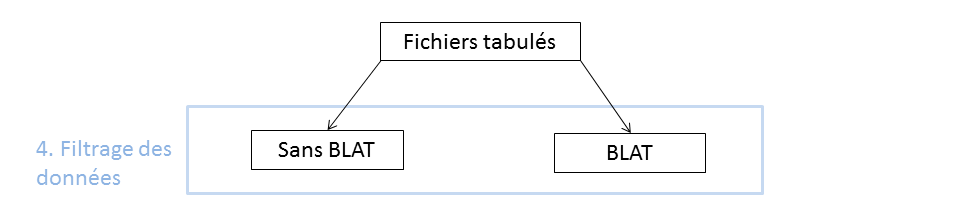
\includegraphics[scale = 0.6]{Figures/partie4.png}
\caption{Filtrage des données}
\label{fig:part4}
\end{figure}

\section{Caractérisation des variations}

Les données filtrées contiendront un nombre minimum de \og faux positifs\fg. Une étude plus approfondie des TFBS pourra alors être envisagée.

Dans un premier temps, il faudra récupérer les TFBS porteurs d'une variation, un shell script sera réalisé pour ce faire.

Les facteurs de transcriptions agissent généralement sur des gènes proches de leur TFBS. En utilisant la base de données \textit{\textbf{RefSeq}} et l'outil \textit{\textbf{intersect}} du logiciel \textbf{Bedtools}, il sera possible de récupérer le ou les gènes les plus proche de chacun des TFBS mutés. 

Les bases de données \textit{\textbf{TRANSFAC}} et \textit{\textbf{CHEA}} disponibles sur le site web \textbf{Harmonizome} \citep{harmonizome} contiennent les gènes cibles des facteurs de transcription. Ces bases pourront être utilisés pour extraire les gènes cibles du jeu de gènes obtenus avec \textbf{Bedtools}.

L'analyse des valeurs de d'expression normalisées en FPKM permettra par la suite de savoir si les gènes, qu'ils soient cible ou pas, ont un changement d'expression. 
 


